\documentclass[12pt]{../manual}
%____________________________________________________________________________
%
%	READ BEFORE USING
%____________________________________________________________________________
%
% This file will not compile unless all the necessary figures are in subfolder named
% "figures" in the same directory as this file. Note that the first time you compile
% this file in a new computer, the references to the figures will all be ???. You
% will have to compile at least three times for all the references to be correct.
% Lastly, take care to not change/remove anything from above this notice. There is
% no guarantee this will compile without all of the definitions and imports above.
%____________________________________________________________________________
%
%	TITLE AND TABLE OF CONTENTS
%____________________________________________________________________________
\begin{document}
\makeheader{Lab 3}{Fall 2019} % Change Semester and Year as needed
\begin{center}
\textbf{\huge ECE 230L - LAB 3}\\~\\
\textbf{\large INTRODUCTION TO CIRCUIT SIMULATION USING PSPICE}\\~\\
\rule{6.5in}{0.5mm}\\
\end{center}

\tableofcontents

\listoffigures

\newpage
%____________________________________________________________________________
%
%	BODY
%____________________________________________________________________________
\section{Objectives of this Laboratory}
The objectives of this laboratory session are to introduce you to the basics of PSpice by learning:
\begin{itemize}
\item How to set-up your PSpice simulation environment,
\item How to represent the circuit elements,
\item How to construct the circuits, and
\item How to simulate the circuits.
\end{itemize}
%____________________________________________________________________________
%
% 	ORCAD
%____________________________________________________________________________
\section{Setting Up a Circuit Using ORCAD Capture}
To create a circuit in a PSpice environment, one must first launch ORCAD:
\begin{enumerate}
\item Open ORCAD Capture CIS
\item Create a new project by selecting {\bf File} $\to$ {\bf New} $\to$ {\bf Project}
\item Name your project `Lab 3'
\item Choose {\bf Analog or Mixed A/D} under the {\bf Create a New Project Using} menu
\item Select {\bf Create a blank project} when prompted
\end{enumerate}

\begin{myfigure}[label=fig:blankSchematic]{Blank Schematic}{Blank Schematic}
\centering
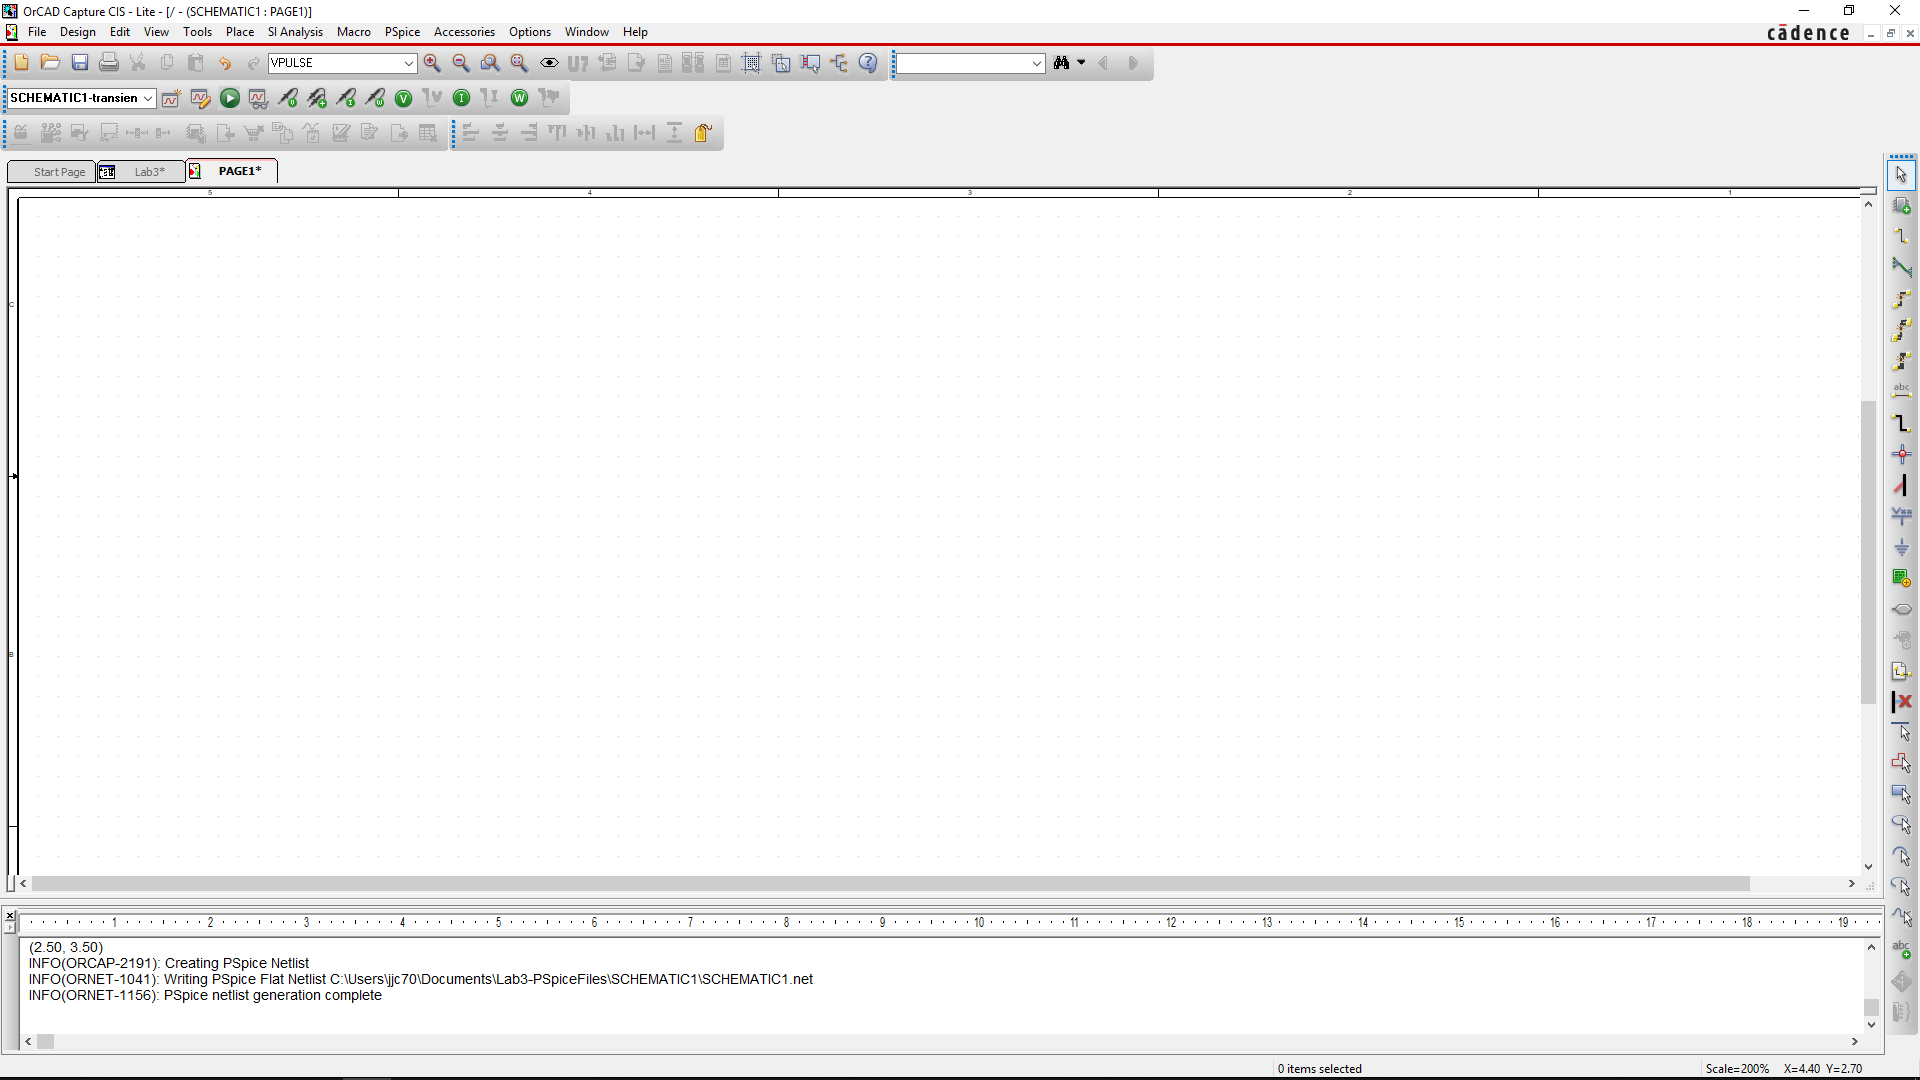
\includegraphics[width=0.9\textwidth]{./figures/BlankSchematic.PNG}
\end{myfigure}

Once the new project has been created, circuit design can begin. Sources, components, ground nodes, and wires can be selected using the {\bf Place} menu.

PSpice will be used to model the circuit in Figure \ref{fig:exampleCircuit} and perform DC, AC, and transient analysis on the circuit.

\begin{myfigure}[label=fig:exampleCircuit]{Example Circuit}{Example Circuit}
\centering
\begin{circuitikz}[scale=2]
\ctikzset{resistors/scale=1.5,batteries/scale=1.5,grounds/scale=2.0,diodes/scale=1.5}
\draw
(0,0) 	to[short] 		++(2,0)
		node[ground] {}
		to[short] 		++(2,0)
		to[C, l_=${C = \SI{1}{\nano\farad}}$]			++(0,2)
		to[short]		++(-2,0)
		to[R, l_=${R_1 = \SI{1}{\kilo\ohm}}$]			++(-2,0)
		to[battery, l_=$v_{in}$]		++(0,-2)
(2,0)	to[R, *-*, l_=${R_2 = \SI{1}{\kilo\ohm}}$]		++(0,2)
;\end{circuitikz}
\end{myfigure}

To make the circuit, 
\begin{enumerate}
\item Add a DC Voltage Source by following \fbox{Place} $\to$ \fbox{PSPice Component} $\to$ \fbox{Source} $\to$ \fbox{Voltage Source} $\to$ \fbox{DC}
\end{enumerate}

Add a DC voltage source to the circuit by following Place $\to$ PSpice Component $\to$ Source $\to$ Voltage Sources $\to$ DC. After adding the voltage source to the schematic, use the Place $\to$ PSpice Components $\to$ Passives menu to insert the remaining resistors and capacitors. Use Ctrl-R to rotate the components. Use Place $\to$ Wire to connect the circuit nodes. To change values of circuit elements, double click on the element and adjust the desired properties. Finally, add a ground node to the circuit schematic. Follow Place $\to$ Ground and select 0/SOURCE as your ground node.
%____________________________________________________________________________
%
%	DC Analysis
%____________________________________________________________________________
\newpage
\section{DC Analysis in PSpice}
To perform a DC analysis of the circuit, you will create a new simulation profile. To create a new profile select \textbf{PSpice} $\to$ \textbf{New Simulation Profile}. Name the new profile `dc' and press \textbf{Create}. To analyze the example circuit, select \textbf{DC Sweep} in the \textbf{Analysis Type} drop down menu and use the following parameters:
\begin{itemize}
\item Sweep variable > Voltage source: V1
\item Sweep Type: Linear
\item Start Value: 0
\item End Value: 10
\item Increment: 0.01
\end{itemize}
Press \textbf{Apply} and \textbf{OK} to save the profile settings. Begin the simulation by selecting \textbf{PSpice} $\to$ \textbf{Run}. To view the circuit behavior at a particular point, follow \textbf{Trace} $\to$ \textbf{Add Trace} to select different values to plot. Plot V(R1:1), V(R1:2), I(R1), and I(R2). Figure \ref{fig:exampleCircuit} shows the circuit schematic and Figure \ref{fig:DCAnalRes} shows the result of DC analysis (top plot: current, bottom plot: voltage).

\begin{myfigure}[label=fig:DCAnalRes]{Result of DC Analysis}{Result of DC Analysis}
\centering
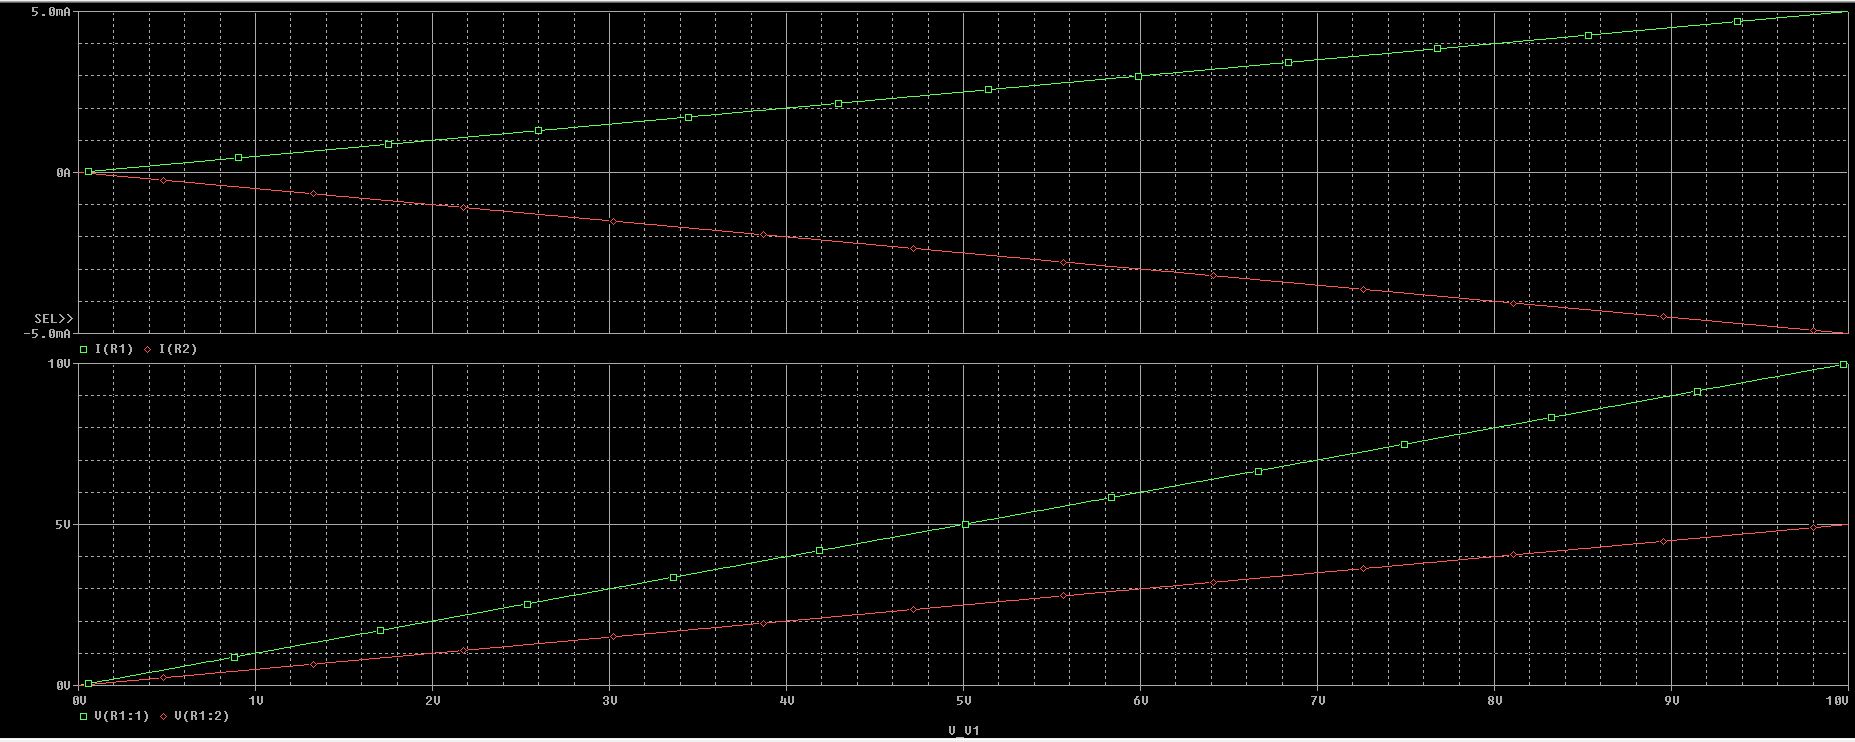
\includegraphics[width=0.9\textwidth]{figures/ResultDCAnalysisCrop.PNG}
\end{myfigure}
%____________________________________________________________________________
%
%	AC Analysis
%____________________________________________________________________________
\newpage
\section{AC Analysis in PSpice}
Before performing an AC analysis a new AC voltage source has to replace the DC source. To change the source, delete the DC source and follow \textbf{Place} $\to$ \textbf{PSpice Component} $\to$ \textbf{Source} $\to$ \textbf{AC}. We include the circuit in Figure \ref{fig:acCircuit}. The following parameters will be used: 
\begin{itemize}
\item DC Value: 10
\item AC Amplitude: 1
\end{itemize}

\begin{myfigure}[colback=white,label=fig:acCircuit]{Circuit for AC Analysis}{Circuit for AC Analysis}
\centering
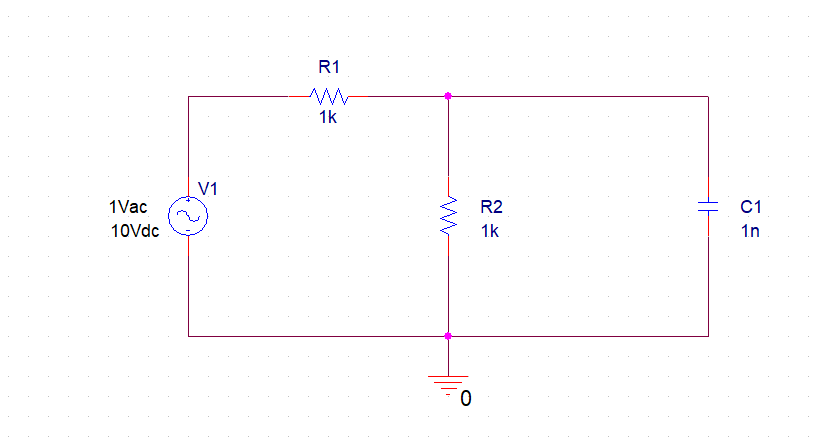
\includegraphics[width=0.9\textwidth]{figures/ACAnalysisCircuitCrop.PNG}
\end{myfigure}

After the voltage source properties have been changed, AC analysis can be performed. First, create a new simulation profile called `ac'. Next, select \textbf{AC Sweep/Noise} in the \textbf{Analysis Type} drop down menu and use the following parameters:
\begin{itemize}
\item AC Sweep Type: Logarithmic 
\begin{itemize}
\item Select \textbf{Decade} from drop down box below
\end{itemize}
\item Start Frequency: 1k
\item Stop Frequency: 1Meg
\item Number of Points per Decade: 10
\end{itemize}
Press \textbf{Apply} and \textbf{OK} to save the profile settings. Begin the simulation by selecting \textbf{PSpice} $\to$ \textbf{Run}.

A screencap of the settings for the AC Analysis is included in Figure \ref{fig:acSettings}.

\begin{myfigure}[label=fig:acSettings]{Settings for AC Analysis}{Settings for AC Analysis}
\centering
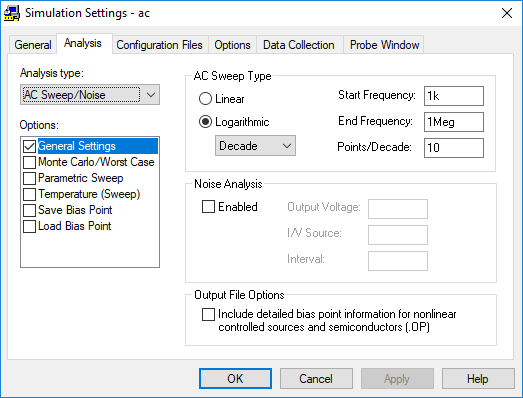
\includegraphics[width=0.6\textwidth]{figures/ACAnalysisSettings.PNG}
\end{myfigure}

\subsection{Trace Expressions in PSpice}

Trace expressions can be used to plot the phase of a desired value, a parameter in units of dB, or plot other useful mathematical operations on circuit parameters. Trace expressions are available under the \textbf{Trace} $\to$ \textbf{Add Trace} menu. Select \textbf{Plot} $\to$ \textbf{Add Plot to Window} and plot the value of V(R2) in dB. Use the trace expression DB(V(R1:2)). Next, add another plot to the window and plot the phase of V(R2). Use the trace expression P(V(R1:2)). The circuit for AC analysis is shown in Figure \ref{fig:acCircuit} and the resulting plots are shown in Figure \ref{fig:acAnalRes}.

\begin{myfigure}[label=fig:acAnalRes]{Result of AC Analysis}{Result of AC Analysis. Top to bottom: V(R1:2), DB(V(R1:2)), P(V(R1:2)).}
\centering
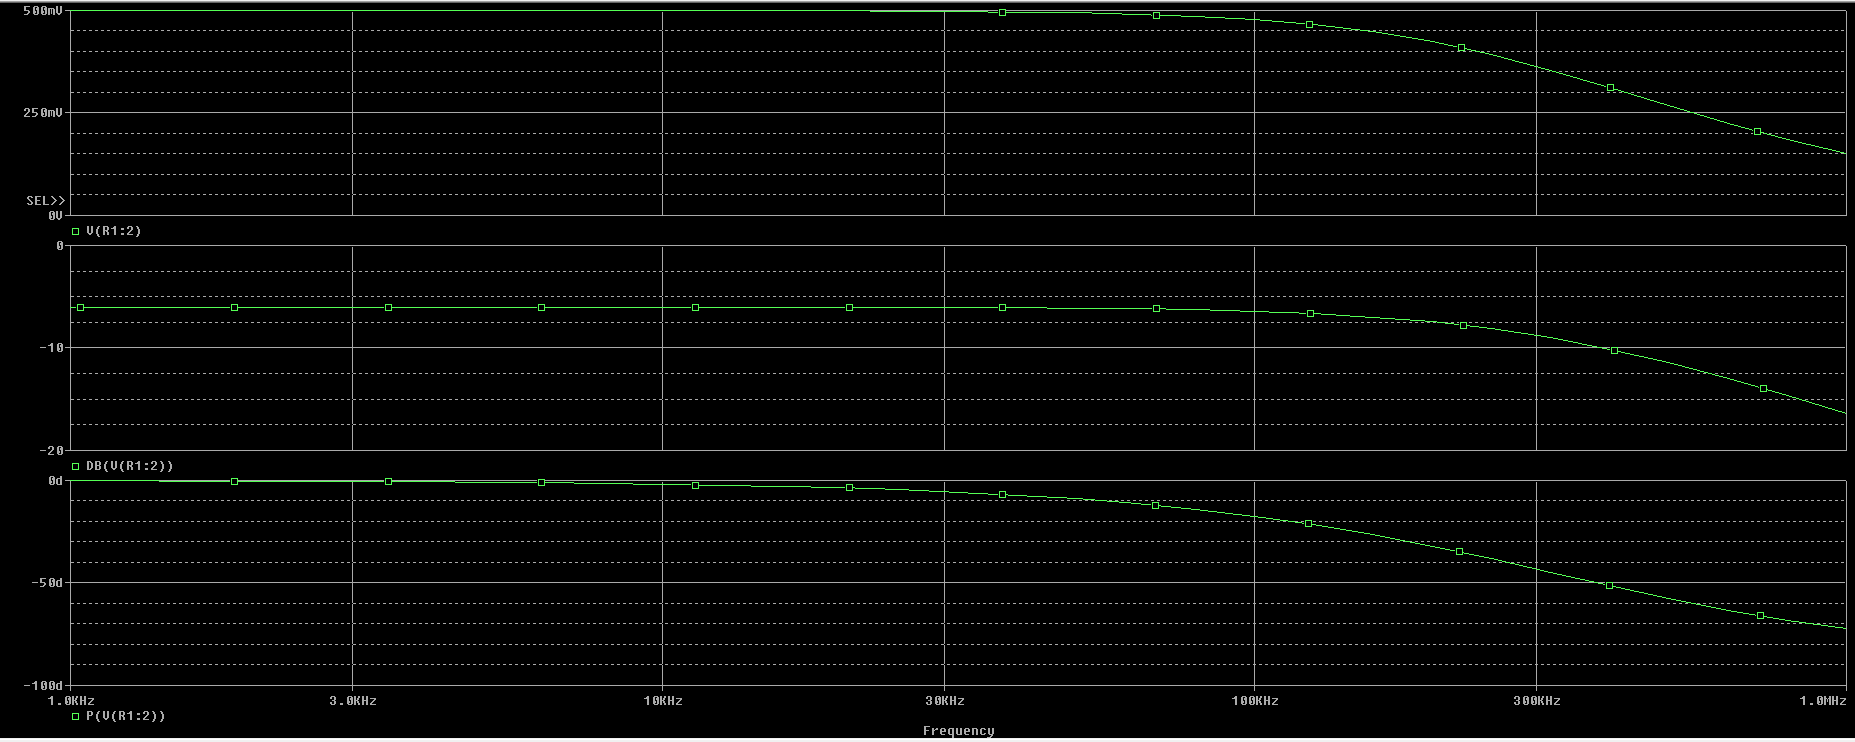
\includegraphics[width=0.9\textwidth]{figures/ResultACAnalysisCrop.PNG}
\end{myfigure}
%____________________________________________________________________________
%
%	Transient Analysis
%____________________________________________________________________________
\section{Transient Analysis in PSpice}

Before performing a transient analysis replace the AC source with a Pulse source (Place-> PSpice Component-> Source-> Pulse). The following parameters will be used to set up the pulse:
\begin{itemize}
\item V1: 0
\item V2: 5
\item TD: 10n
\item TR: 20n
\item TF: 20n
\item PW: 500n
\item PER: 2u
\end{itemize}

\begin{myfigure}[colback=white,label=fig:trans]{Circuit for Transient Analysis}{Circuit for Transient Analysis}
\centering
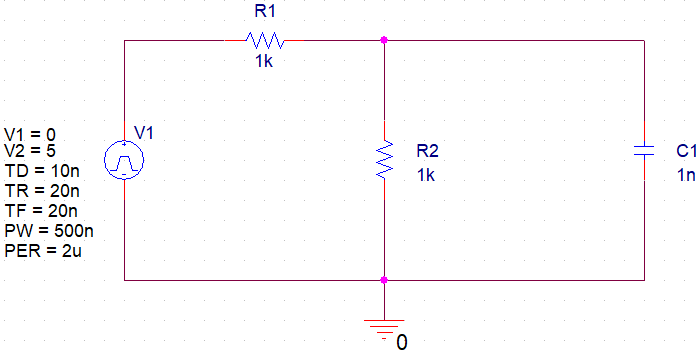
\includegraphics[width=0.9\textwidth]{figures/TransientAnalysisCircuitCrop.PNG}
\end{myfigure}


Create a new simulation profile called ?Transient?. To analyze the example circuit, select ?Time Domain (Transient)? in the Analysis Type drop down menu and use the following parameters:
? Run to Time: 2u
? Start saving data after: 0
? Maximum step size: 10n
Press ?Apply? and ?OK? to save the profile settings. Begin the simulation by selecting PSpice-> Run. To view the circuit behavior at a particular point, follow Trace-> Add Trace to select different values to plot or use the voltage and current markers indicated in Figure 1. Plot the source voltage and V(R2). The circuit for transient analysis is shown in figure 7 and the resulting plot is shown in figure 8.

\begin{myfigure}[label=fig:transAnalRes]{Result of Transient Analysis}{Result of Transient Analysis}
\centering
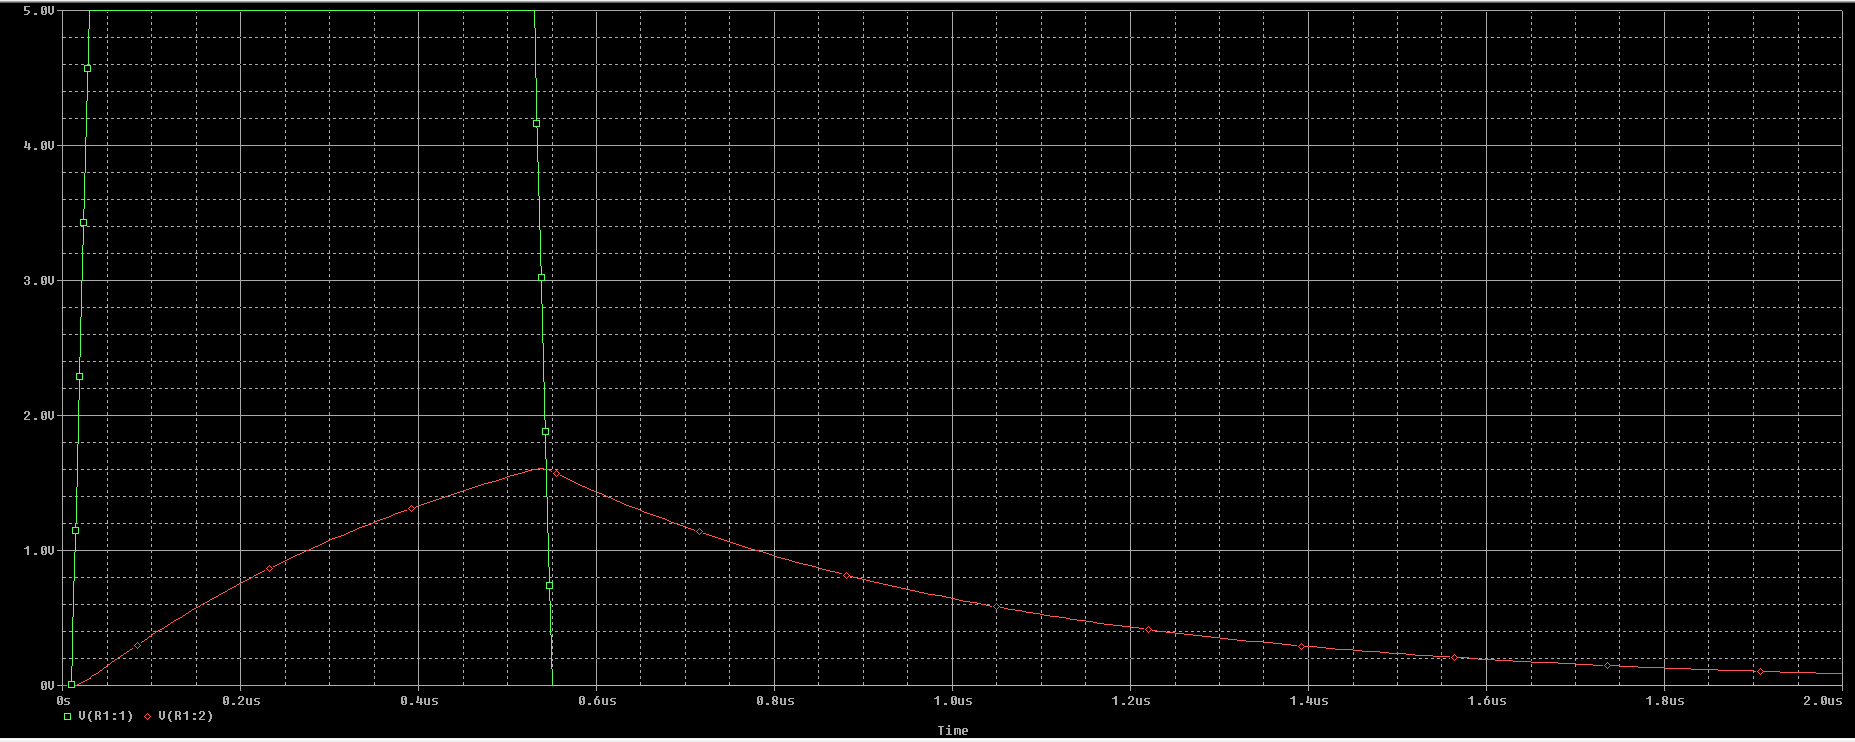
\includegraphics[width=0.9\textwidth]{figures/ResultTransientAnalysisCrop.PNG}
\end{myfigure}
%____________________________________________________________________________
%
%	Practice Example
%____________________________________________________________________________
\section{Practice Example}

\begin{myfigure}[label=fig:practice]{Practice Circuit}{Practice Circuit}
\centering
\begin{circuitikz}[scale=2]
\ctikzset{resistors/scale=1.5,batteries/scale=1.5,grounds/scale=2.0,diodes/scale=1.5}
\draw
(0,0) 	to[short, *-] 	++(0,1)
		to[C, l=${C_1=\SI{1}{\nano\farad}}$]	++(2,0)
		to[short, -*]	++(0,-1)
		to[short]		++(1,0)
		to[R, l=${R_{sec}=\SI{1}{\kilo\ohm}}$] 	++(0,-2)
		to[short, -*]		++(-2,0)
		node[ground] {}
		to[short]		++(-2,0)
(2,0)	to[R, l=${R_{fir}=\SI{1}{\kilo\ohm}}$] 	++(-2,0)
		to [short] ++ (-1,0)
		to[battery, l_=${v_{IN}}$, i=${i_{IN}}$] 	++(0,-2)
;\end{circuitikz}
\end{myfigure}
%____________________________________________________________________________
%
%	Exploration
%____________________________________________________________________________
\section{Exploration: Th\'evenin Equivalent Circuits}
\subsection{Purpose}
The purpose of this exercise is to learn how to form a Th\'evenin Equivalent circuit by using circuit parameters obtained during simulation.

\subsection{Introduction}
Any linear DC circuit as seen at a pair of terminals can be reduced to a practical voltage source (an ideal voltage source in series with a resistor).

\begin{myfigure}[label=fig:thev]{Th\'evenin Equivalent Circuit}{Th\'evenin Equivalent Circuit}
\centering
\begin{circuitikz}[scale=2]
\ctikzset{resistors/scale=1.5,batteries/scale=1.5,grounds/scale=2.0,diodes/scale=1.5}
\draw
(0,0)	to[R, *-, l=${R_{TH}}$]		++(-4,0)
		to[battery, l=${V_{OC}}$] 	++(0,-2)
		to[short, -*]	++(4,0)
(0,0.25)	node[] {A}
(0,-1.75)	node[] {B}
;\end{circuitikz}
\end{myfigure}

To form a Th\'evenin Equivalent circuit, two quantities must be calculated, measured, or simulated:
\begin{enumerate}
\item $v_{oc}$: The open circuit voltage drop from terminals A to B
\item $i_{sc}$: The short circuit current from terminals A to B
\end{enumerate}
Once the values for $v_{oc}$ and $i_{sc}$ have been obtained, the Th\'evenin resistance $R_{TH}$ can be determined using the relation:
\begin{align}
R_{TH} = \frac{v_{oc}}{i_{sc}}
\end{align}
If the circuit contains no dependent sources, then $R_{TH}$ may also be found by turning off all of the independent sources and using resistance reduction at terminals A and B.

\subsection{Exercise}
You will simulate the circuit in figure 11 and form its Th\'evenin Equivalent circuit as seen at a pair of terminals.
\subsection{Practice Exercise: Th\'evenin Equivalent Circuit}
%____________________________________________________________________________
%
%	Grading Rubric
%____________________________________________________________________________
\newpage
\phantomsection % needed in order to link from table of contents to here
\section*{Grading Rubric}
\addcontentsline{toc}{section}{Grading Rubric} % adds section*{} to table of contents
\markboth{Grading Rubric}{Grading Rubric}
\vfill % used to center table vertically on page
\begin{table}[ht!]
\caption{ECE 230L Laboratory 3 Grading Rubric}
\centering
\begin{tabular}{l|c} \hline
Criteria & Points Possible \\ \hline \hline
\textbf{DC Analysis}			& \textbf{10} \\
Circuit Diagram 				& 5 \\
Waveforms 						& 5 \\ \hline
\textbf{AC Analysis}			& \textbf{10} \\
Circuit Diagram 				& 5 \\
Waveforms 						& 5 \\ \hline
\textbf{Transient Analysis}		& \textbf{10} \\
Circuit Diagram 				& 5 \\ 
Waveforms 						& 5 \\ \hline
\textbf{Practice Exercise}		& \textbf{35} \\
Circuit Diagram 				& 5 \\
DC Analysis						& 10 \\
AC Analysis						& 10 \\
Transient Analysis				& 10 \\ \hline
\textbf{Th\'evenin Equivalent Example Circuit} & \textbf{20} \\
Circuit Diagram					& 10 \\
$V_{OC}$ and $I_{SC}$ Labeled	& 5 \\
Correct $R_{TH}$ Value			& 5 \\ \hline
\textbf{Th\'evenin Equivalent Challenge Circuit} & \textbf{15} \\
Circuit Diagram					& 5 \\
$V_{OC}$ and $I_{SC}$ Labeled	& 5 \\
Correct $R_{TH}$ Value			& 5 \\ \hline \hline
Total							& 100 \\ \hline
\end{tabular}
\end{table}
\vfill % used to center table vertically on page
\end{document}
